%% LyX 2.0.6 created this file.  For more info, see http://www.lyx.org/.
%% Do not edit unless you really know what you are doing.
\documentclass[oneside,spanish,english,french,brazil,12pt,openright,twoside,a4paper,english,french,spanish,brazil]{abntex2}
\usepackage[T1]{fontenc}
\usepackage[utf8]{inputenc}
\setcounter{secnumdepth}{3}
\setcounter{tocdepth}{3}
\usepackage{verbatim}
\usepackage{float}
\usepackage{url}
\usepackage{pdfpages}
\usepackage[authoryear]{natbib}

\makeatletter

%%%%%%%%%%%%%%%%%%%%%%%%%%%%%% LyX specific LaTeX commands.
\providecommand{\LyX}{L\kern-.1667em\lower.25em\hbox{Y}\kern-.125emX\@}
%% Because html converters don't know tabularnewline
\providecommand{\tabularnewline}{\\}
%% A simple dot to overcome graphicx limitations
\newcommand{\lyxdot}{.}


%%%%%%%%%%%%%%%%%%%%%%%%%%%%%% User specified LaTeX commands.
% ---
% PACOTES
% ---
\usepackage{lastpage}			% Usado pela Ficha catalográfica
\usepackage{indentfirst}		% Indenta o primeiro parágrafo de cada seção.
\usepackage{color}				% Controle das cores

% ---
% Pacotes adicionais, usados apenas no âmbito do Modelo Canônico do abnteX2
% ---
\usepackage{lipsum}				% para geração de dummy text
% ---

% ---
% Pacotes de citações
% ---
\usepackage[brazilian,hyperpageref]{backref}	 % Paginas com as citações na bibl
\usepackage[alf]{abntex2cite}	% Citações padrão ABNT

% --- 
% CONFIGURAÇÕES DE PACOTES
% --- 

% ---
% Configurações do pacote backref
% Usado sem a opção hyperpageref de backref
\renewcommand{\backrefpagesname}{Citado na(s) página(s):~}
% Texto padrão antes do número das páginas
\renewcommand{\backref}{}
% Define os textos da citação
\renewcommand*{\backrefalt}[4]{
\ifcase #1
Nenhuma citação no texto.
\or
Citado na página #2.
\else
Citado #1 vezes nas páginas #2.
\fi}

% --- 
% Espaçamentos entre linhas e parágrafos 
% --- 

% O tamanho do parágrafo é dado por:
\setlength{\parindent}{1.3cm}

% Controle do espaçamento entre um parágrafo e outro:
\setlength{\parskip}{0.2cm}  % tente também \onelineskip

% ---
% compila o indice
% ---
\makeindex
% ---

\makeatother

\usepackage{babel}
\makeatletter
\addto\shorthandsspanish{\spanishdeactivate{~<>}}

\addto\extrasfrench{%
   \providecommand{\og}{\leavevmode\flqq~}%
   \providecommand{\fg}{\ifdim\lastskip>\z@\unskip\fi~\frqq}%
}

\makeatother
\begin{document}
\begin{comment}
Os valores colocados nos campos abaixo \textbf{não serão impressos}
ao gerar o documento final. Esses campos somente modificam os valores
para as macros do documento, as quais serão usadas posteriormente
dentro do esqueleto da tese. Esta parte do documento é como se fosse
a ``ficha cadastral'' da tese.
\end{comment}



\titulo{Modelo Canônico de\\
Trabalho Acadêmico com abn\TeX{}2 e \LyX{}}




\local{Universidade do Brasil -- UBr\\
Faculdade de Arquitetura da Informação\\
Programa de Pós-Graduação}




\data{6 de Junho de 2013}




\autor{Paulo Afonso Graner Fessel}


\orientador{Lauro César Araújo}


\coorientador{Sérgio Granja}


\coorientador[Co-Orientadores]{Equipe abn\TeX{}}


\tipotrabalho{Dissertação de Mestrado}

\begin{comment}
A partir daqui, inicia-se o texto impresso
\end{comment}


\frenchspacing

\pretextual

\imprimircapa

\imprimirfolhaderosto*{}
\begin{fichacatalografica}
\sffamily

\vspace*{\fill}
\begin{minipage}[c][12.5cm]{1\textwidth}%
\rule[0.5ex]{1\textwidth}{1pt}

\imprimirautor

\hspace{0.5cm}\imprimirtitulo / \imprimirautor. -- \imprimirlocal,
\imprimirdata-

\hspace{0.5cm}\pageref{LastPage} p. il. (algumas color.) ; 30 cm.

\hspace{0.5cm}\imprimirorientadorRotulo~\imprimirorientador\\


\parbox[c][1\totalheight][t]{1\textwidth}{%
\hspace{0.5cm}\imprimirtipotrabalho~--~\imprimirinstituicao,
\imprimirdata.\\


\hspace{0.5cm}1. Palavra-chave1. 2. Palavra-chave2. I. Orientador.
II. Universidade xxx. III. Faculdade de xxx. IV. Título\\


\hspace{8.75cm} CDU 02:141:005.7%
}

\rule[0.5ex]{1\textwidth}{1pt}%
\end{minipage}\end{fichacatalografica}
\begin{errata}
Elemento opcional da \citeauthor{NBR14724:2001}. Exemplo:\\
\\
FERRIGNO, C. R. A. \textbf{Tratamento de neoplasias ósseas apendiculares
com reimplantação de enxerto ósseo autólogo autoclavado associado
ao plasma rico em plaquetas}: estudo crítico na cirurgia de preservação
de membro em cães. 2011. 128 f. Tese (Livre-Docência) - Faculdade
de Medicina Veterinária e Zootecnia, Universidade de São Paulo, São
Paulo, 2011.

\begin{center}
\begin{tabular}{|l|l|l|l|}
\hline 
\textbf{Folha} & \textbf{Linha} & \textbf{Onde se lê} & \textbf{Leia-se}\tabularnewline
\hline 
\hline 
1 & 10 & auto-conclavo & autoconclavo\tabularnewline
\hline 
\end{tabular}
\par\end{center}\end{errata}
\begin{folhadeaprovacao}
\includepdf[pages=1]{\lyxdot \lyxdot /\lyxdot \lyxdot /\lyxdot \lyxdot /\lyxdot lyx/templates/FolhaDeAprovacao}\end{folhadeaprovacao}
\begin{dedicatoria}
\begin{center}
\vspace*{\fill}
\textit{Este trabalho é dedicado às crianças adultas que,}\\
\textit{ quando pequenas, sonharam em se tornar cientistas.}
\par\end{center}

\vspace*{\fill}
\end{dedicatoria}
\begin{agradecimentos}
Os agradecimentos principais são direcionados à Gerald Weber, Miguel
Frasson, Leslie H. Watter, Bruno Parente Lima, Flávio de Vasconcellos
Corrêa, Otavio Real Salvador, Renato Machnievscz%
\footnote{Os nomes dos integrantes do primeiro projeto \abnTeX foram extraídos
de \url{http://codigolivre.org.br/projects/abntex/}%
} e todos aqueles que contribuíram para que a produção de trabalhos
acadêmicos conforme as normas ABNT com \LaTeX{} fosse possível.

Agradecimentos especiais são direcionados ao Centro de Pesquisa em
Arquitetura da Informação%
\footnote{\url{http://www.cpai.unb.br/}%
} da Universidade de Brasília (CPAI), ao grupo de usuários \textbf{latex-br}%
\footnote{\url{http://groups.google.com/group/latex-br}%
} e aos novos voluntários do grupo abn\TeX{}2 %
\footnote{\url{http://groups.google.com/group/abntex2} e \url{http://abntex2.googlecode.com/}%
} que contribuíram e que ainda contribuirão para a evolução do abn\TeX{}.\end{agradecimentos}
\begin{epigrafe}
\begin{flushright}
\vspace*{\fill}
\textit{``Não vos amoldeis às estruturas deste mundo,}\\
\textit{mas transformai-vos pela renovação da mente,}\\
\textit{a fim de distinguir qual é a vontade de Deus:}\\
\textit{o que é bom, o que Lhe é agradável, o que é perfeito}.\\
(Bíblia Sagrada, Romanos 12, 2)
\par\end{flushright}\end{epigrafe}
\begin{resumo}
\noindent Segundo a \citeauthor[3.1-3.2][]{NBR6028:2003}, ``o resumo
deve ressaltar o objetivo, o método, os resultados e as conclusões
do documento. A ordem e a extensão destes itens dependem do tipo de
resumo (informativo ou indicativo) e do tratamento que cada item recebe
no documento original. O resumo deve ser precedido da referência do
documento, com exceção do resumo inserido no próprio documento. (\ldots{})
As palavras-chave devem figurar logo abaixo do resumo, antecedidas
da expressão Palavras-chave:, separadas entre si por ponto e finalizadas
também por ponto''.

\noindent \textbf{Palavras-chaves:} latex. abntex. editoração de texto.
\end{resumo}
\cleardoublepage{}
\begin{resumo}[Abstract]
\noindent \foreignlanguage{english}{This is the english abstract.}

\selectlanguage{english}%
\noindent \textbf{Key words:} latex. abntex. text typesetting.
\end{resumo}
\cleardoublepage{}
\begin{resumo}[Résumé]
\noindent \foreignlanguage{french}{Ce texte-ci c'est le résumé en
français.}

\selectlanguage{french}%
\noindent \textbf{Mots-clés:} latex. abntex. publication de textes.
\end{resumo}
\cleardoublepage{}
\selectlanguage{spanish}%
\begin{resumo}[Resumen]
\noindent Este es el resumen en español.

\noindent \textbf{Palavras clave: }latex. abntex. publicación de textos.
\end{resumo}
\selectlanguage{brazil}%
\cleardoublepage{}

\listoffigures


\cleardoublepage{}

\listoftables
\cleardoublepage{}

\tableofcontents*

\cleardoublepage{}


\chapter*{Introdução}

Este documento e seu código-fonte são exemplos de referência de uso
da classe abntex2 e do pacote abntex2cite. O documento exemplifica
a elaboração de trabalho acadêmico (tese, dissertação e outros do
gênero) produzido conforme a ABNT NBR 14724:2011 \textbf{Informação
e documentação - Trabalhos acadêmicos - Apresentação}.

A expressão ``Modelo Canônico'' é utilizada para indicar que abn\TeX{}
não é modelo específico de nenhuma universidade ou instituição, mas
que implementa tão somente os requisitos das normas da ABNT. Uma lista
completa das normas observadas pelo abn\TeX{} é apresentada em \citealp{abntex2classe}.

Sinta-se convidado a participar do projeto abn\TeX{}! Acesse o site
do projeto em \url{http://abntex2.googlecode.com/}. Também fique
livre para conhecer, estudar, alterar e redistribuir o trabalho do
abn\TeX{}, desde que os arquivos modificados tenham seus nomes alterados
e que os créditos sejam dados aos autores originais, nos termos da
``The \LaTeX{} Project Public License''%
\footnote{\url{http://abntex2.googlecode.com/}%
}.

Encorajamos que sejam realizadas customizações específicas deste exemplo
para universidades e outras instituições --- como capas, folha de
aprovação, etc. Porém, recomendamos que ao invés de se alterar diretamente
os arquivos do abn\TeX{}, distribua-se arquivos com as respectivas
customizações. Isso permite que futuras versões do abn\TeX{} não se
tornem automaticamente incompatíveis com as customizações promovidas.
Consulte \citeauthor[ "como customizar"]{abntex2-wiki-como-customizar}
para mais informações.

Este documento deve ser utilizado como complemento dos manuais do
abn\TeX{} (\citealp{abntex2classe};\citealp{abntex2cite};\citealp{abntex2cite-alf})
e da classe \textsf{memoir}\citep{memoir}. 

Esperamos, sinceramente, que o abn\TeX{} aprimore a qualidade do trabalho
que você produzirá, de modo que o principal esforço seja concentrado
no principal: na contribuição científica.

Equipe abn\TeX{} 

Lauro César Araujo


\part{Preparação da pesquisa}



%% LyX 2.0.6 created this file.  For more info, see http://www.lyx.org/.
%% Do not edit unless you really know what you are doing.
\documentclass[oneside,spanish,english,french,brazil,12pt,openright,twoside,a4paper,english,french,spanish,brazil]{abntex2}
\usepackage[T1]{fontenc}
\usepackage[utf8]{inputenc}
\setcounter{secnumdepth}{3}
\setcounter{tocdepth}{3}
\usepackage{array}
\usepackage{longtable}
\usepackage{prettyref}
\usepackage{float}
\usepackage{textcomp}
\usepackage{url}
\usepackage{graphicx}
\PassOptionsToPackage{normalem}{ulem}
\usepackage{ulem}
\usepackage{nameref}

\makeatletter

%%%%%%%%%%%%%%%%%%%%%%%%%%%%%% LyX specific LaTeX commands.

\let\pr@chap=\pr@cha
\providecommand{\LyX}{L\kern-.1667em\lower.25em\hbox{Y}\kern-.125emX\@}
%% Because html converters don't know tabularnewline
\providecommand{\tabularnewline}{\\}
%% A simple dot to overcome graphicx limitations
\newcommand{\lyxdot}{.}


%%%%%%%%%%%%%%%%%%%%%%%%%%%%%% Textclass specific LaTeX commands.
\newenvironment{lyxcode}
{\par\begin{list}{}{
\setlength{\rightmargin}{\leftmargin}
\setlength{\listparindent}{0pt}% needed for AMS classes
\raggedright
\setlength{\itemsep}{0pt}
\setlength{\parsep}{0pt}
\normalfont\ttfamily}%
 \item[]}
{\end{list}}

%%%%%%%%%%%%%%%%%%%%%%%%%%%%%% User specified LaTeX commands.
% ---
% PACOTES
% ---
\usepackage{lastpage}			% Usado pela Ficha catalográfica
\usepackage{indentfirst}		% Indenta o primeiro parágrafo de cada seção.
\usepackage{color}				% Controle das cores
\usepackage[figurewithin=none]{caption}
% ---
% Pacotes adicionais, usados apenas no âmbito do Modelo Canônico do abnteX2
% ---
\usepackage{lipsum}				% para geração de dummy text
% ---

% ---
% Pacotes de citações
% ---
\usepackage[brazilian,hyperpageref]{backref}	 % Paginas com as citações na bibl
\usepackage[alf]{abntex2cite}	% Citações padrão ABNT

% --- 
% CONFIGURAÇÕES DE PACOTES
% --- 

% ---
% Configurações do pacote backref
% Usado sem a opção hyperpageref de backref
\renewcommand{\backrefpagesname}{Citado na(s) página(s):~}
% Texto padrão antes do número das páginas
\renewcommand{\backref}{}
% Define os textos da citação
\renewcommand*{\backrefalt}[4]{
\ifcase #1 %
Nenhuma citação no texto.%
\or
Citado na página #2.%
\else
Citado #1 vezes nas páginas #2.%
\fi}%
% ---

% --- 
% Espaçamentos entre linhas e parágrafos 
% --- 

% O tamanho do parágrafo é dado por:
\setlength{\parindent}{1.3cm}

% Controle do espaçamento entre um parágrafo e outro:
\setlength{\parskip}{0.2cm}  % tente também \onelineskip

% ---
% compila o indice
% ---
\makeindex
% ---

\makeatother

\usepackage{babel}
\makeatletter
\addto\shorthandsspanish{\spanishdeactivate{~<>}}

\addto\extrasfrench{%
   \providecommand{\og}{\leavevmode\flqq~}%
   \providecommand{\fg}{\ifdim\lastskip>\z@\unskip\fi~\frqq}%
}

\makeatother
\begin{document}

\chapter{\label{chap:Resultados-de-comandos}Resultados de comandos}


\chapterprecis{Isto é uma sinopse de capítulo. A ABNT não traz nenhuma normatização
a respeito desse tipo de resumo, que é mais comum em romances e livros
técnicos.}


\section{Codificação dos arquivos: UTF8}

A codificação de todos os arquivos do abn\TeX{}2 é \texttt{UTF8}.
É necessário que você utilize a mesma codificação nos documentos que
escrever, inclusive nos arquivos de base bibliográficas |.bib|. 


\section{Citações diretas}

Utilize o ambiente \texttt{citacao} para incluir citações diretas
com mais de três linhas:


\begin{citacao}
As citações diretas, no texto, com mais de três linhas, devem ser
destacadas com recuo de 4 cm da margem esquerda, com letra menor que
a do texto utilizado e sem as aspas. No caso de documentos datilografados,
deve-se observar apenas o recuo.
\end{citacao}
O ambiente \texttt{citacao} pode receber como parâmetro opcional um
nome de idioma previamente carregado nas opções da classe (\textbackslash{}autoref\{sec-hifenizacao\}).
No \LyX{}, esse parâmetro é ajustado através do comando ``Insert→Short
Title'', sendo que o texto da opção representa o idioma escolhido.
Nesse caso, o texto da citação é automaticamente escrito em itálico
e a hifenização é ajustada para o idioma selecionado na opção do ambiente.
Por exemplo:
\begin{citacao}[english]
Text in English language in italic with correct hyphenation.
\end{citacao}
Citações simples, com até três linhas, devem ser incluídas com aspas.
``Amor é fogo que arde sem se ver''.


\section{Notas de rodapé}

As notas de rodapé são detalhadas pela NBR 14724:2011 na seção 5.2.1%
\footnote{As notas devem ser digitadas ou datilografadas dentro das margens,
ficando separadas do texto por um espaço simples de entre as linhas
e por filete de 5 cm, a partir da margem esquerda. Devem ser alinhadas,
a partir da segunda linha da mesma nota, abaixo da primeira letra
da primeira palavra, de forma a destacar o expoente, sem espaço entre
elas e com fonte menor \textbackslash{}citeonline{[}5.2.1{]}\{NBR14724:2011\}.%
}%
\footnote{Caso uma série de notas sejam criadas sequencialmente, o abn\TeX{}
instrui o \LaTeX{} para que uma vírgula seja colocada após cada número
do expoente que indica a nota de rodapé no corpo do texto.%
}%
\footnote{Verifique se os números do expoente possuem uma vírgula para dividi-los
no corpo do texto.%
}.


\section{Tabelas}

\index{tabelas}

A \ref{tab-nvinv} é um exemplo de tabelas construídas com a interface
gráfica do \LyX{}. Comece inserindo tabelas no texto com o comando
``Insert→Float→Table'' para ter maior flexibilidade:

\begin{table}[H]
\caption{Níveis de investigação}
\label{tab-nvinv}%
\begin{longtable}{>{\raggedright}p{2.6cm}|>{\raggedright}p{6cm}|>{\raggedright}p{2.25cm}|>{\raggedright}p{3.4cm}}
\textbf{Nível de investigação} & \textbf{Insumos} & \textbf{Sistemas de investigação} & \textbf{Produtos}\tabularnewline
\hline 
Meta-nível & Filosofia da ciência & Epistemologia & Paradigma\tabularnewline
\hline 
Nível do objeto & Paradigmas do metanível e evidências do nível inferior & Ciência & Teorias e modelos\tabularnewline
\hline 
Nível inferior & Modelos e métodos do nível do objeto e problemas do nível inferior & Prática & Solução de problemas\tabularnewline
\end{longtable}


\legend{Fonte: \cite{van86}}
\end{table}



\section{Figuras}

Figuras podem ser criadas diretamente em \LaTeX{}, com o uso de ERT
(``Evil Red Text''), como o exemplo da \ref{fig-circulo}.

\begin{center}
\begin{figure}[H]
\caption{A delimitação do espaço}
\label{fig-circulo}

\begin{center}
	\setlength{\unitlength}{5cm} 		
	\begin{picture}(1,1) 		
		\put(0,0){\line(0,1){1}} 		
		\put(0,0){\line(1,0){1}} 		
		\put(0,0){\line(1,1){1}} 		
		\put(0,0){\line(1,2){.5}} 		
		\put(0,0){\line(1,3){.3333}} 		
		\put(0,0){\line(1,4){.25}} 		
		\put(0,0){\line(1,5){.2}} 		
		\put(0,0){\line(1,6){.1667}} 		
		\put(0,0){\line(2,1){1}} 		
		\put(0,0){\line(2,3){.6667}} 		
		\put(0,0){\line(2,5){.4}} 		
		\put(0,0){\line(3,1){1}} 		
		\put(0,0){\line(3,2){1}} 		
		\put(0,0){\line(3,4){.75}} 		
		\put(0,0){\line(3,5){.6}} 		
		\put(0,0){\line(4,1){1}} 		
		\put(0,0){\line(4,3){1}} 		
		\put(0,0){\line(4,5){.8}} 		
		\put(0,0){\line(5,1){1}} 		
		\put(0,0){\line(5,2){1}} 		
		\put(0,0){\line(5,3){1}} 		
		\put(0,0){\line(5,4){1}} 		
		\put(0,0){\line(5,6){.8333}} 		
		\put(0,0){\line(6,1){1}} 		
		\put(0,0){\line(6,5){1}} 		
	\end{picture} 	
\end{center}
\end{figure}

\par\end{center}

Ou então figuras podem ser incorporadas de arquivos externos, como
é o caso da \ref{fig-grafico}. Se a figura que ser incluída se tratar
de um diagrama, um gráfico ou uma ilustração que você mesmo produza,
priorize o uso de imagens vetoriais no formato PDF. Com isso, o tamanho
do arquivo final do trabalho será menor, e as imagens terão uma apresentação
melhor, principalmente quando impressas, uma vez que imagens vetorias
são perfeitamente escaláveis para qualquer dimensão. Nesse caso, se
for utilizar o Microsoft Excel para produzir gráficos, ou o Microsoft
Word para produzir ilustrações, exporte-os como PDF e os incorpore
ao documento conforme o exemplo abaixo. No entanto, para manter a
coerência no uso de software livre (já que você está usando \LaTeX{}
e abn\TeX{}), teste a ferramenta \textsf{InkScape}\index{InkScape}
(\url{http://inkscape.org/}). Ela é uma excelente opção de código-livre
para produzir ilustrações vetoriais, similar ao CorelDraw ou ao Adobe
IllustratorAdobe Illustrator\index{Adobe Illustrator}. De todo modo,
caso não seja possível utilizar arquivos de imagens como PDF, utilize
qualquer outro formato, como JPEG, GIF, BMP, etc. Nesse caso, você
pode tentar aprimorar as imagens incorporadas com o software livre
\textsf{Gimp\index{Gimp}} (\url{http://www.gimp.org}). Ele é uma
alternativa livre ao Adobe Photoshop\index{Photoshop}. Da mesma maneira
que as tabelas, comece inserindo a figura com o comando ``Insert→Float→Figure''.

\begin{center}
\begin{figure}[H]
\caption{Gráfico produzido em excel e salvo como PDF}
\label{fig-grafico}

\noindent \begin{centering}
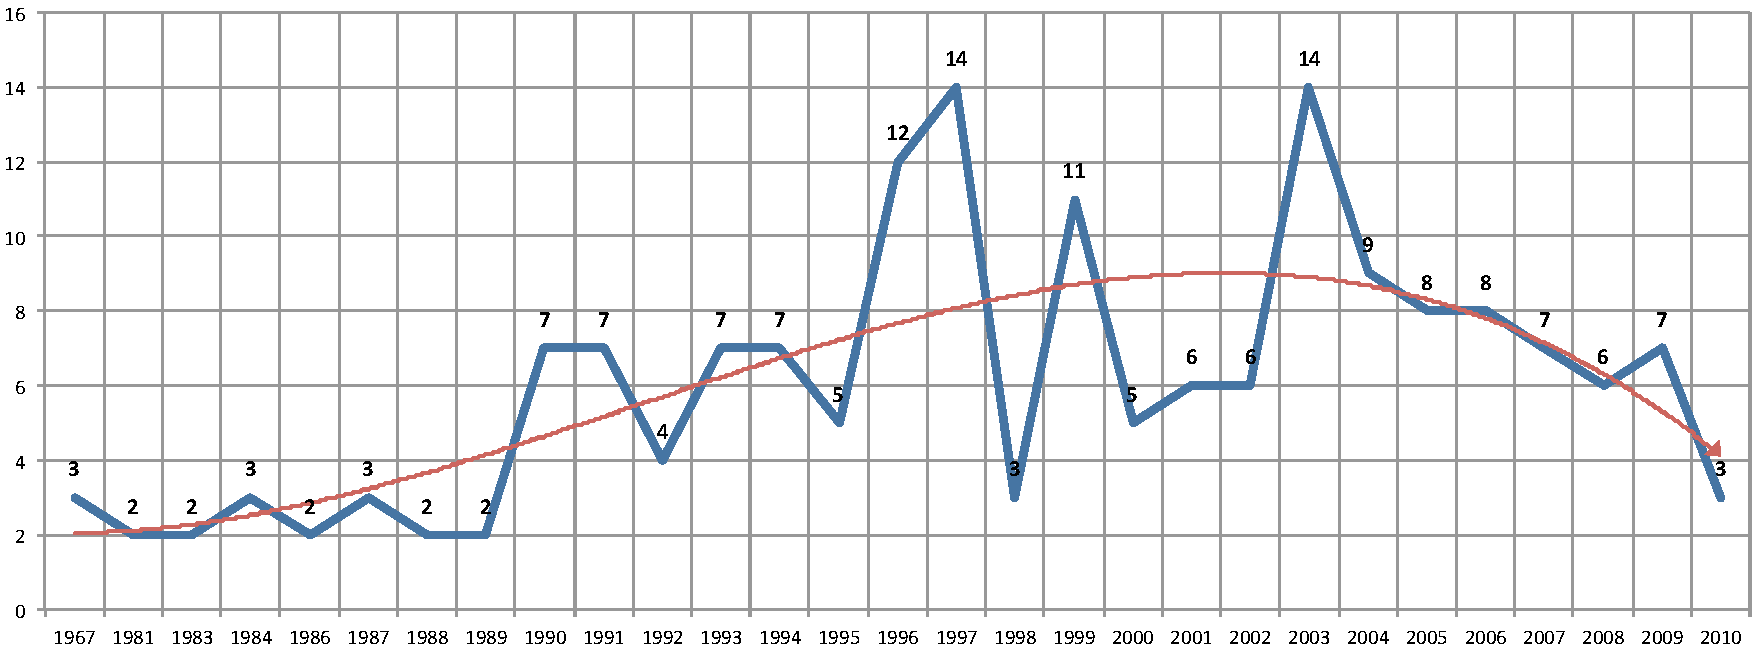
\includegraphics[clip,scale=0.5]{/home/pfessel/abntex2/doc/latex/abntex2/abntex2-modelo-img-grafico}
\par\end{centering}


\legend{Fonte: \cite[p. 24]{araujo2012}}

\end{figure}

\par\end{center}


\subsection{Figuras em \textsf{\emph{minipages}}}

\textsf{\emph{Minipages}} são usadas para inserir textos ou outros
elementos em quadros com tamanhos e posições controladas. No \LyX{}
elas são emuladas com os\linebreak{}
comandos ``Insert→Float→Figure'' e ``Insert→Float→Box''. Um roteiro
completo é dado em no Wiki do \LyX{}, em \url{http://wiki.lyx.org/Examples/FiguresSideBySide};
note que, na tela. os gráficos podem aparecer empilhados e não necessariamente
um do lado do outro. Será necessário também acertar a largura da de
cada minipage manualmente, clicando-se com o botão direito em ``Box(Minipage)''
e escolhendo ``Settings→Width'' e ``Settings→\% Page Width''.
Veja o exemplo da \ref{fig-minipage-grafico1} e da \ref{fig-minipage-grafico2}.

\begin{figure}[H]
\begin{minipage}[t]{0.4\textwidth}%
\caption{Gráfico 1 da minipage}
\label{fig-minipage-grafico1}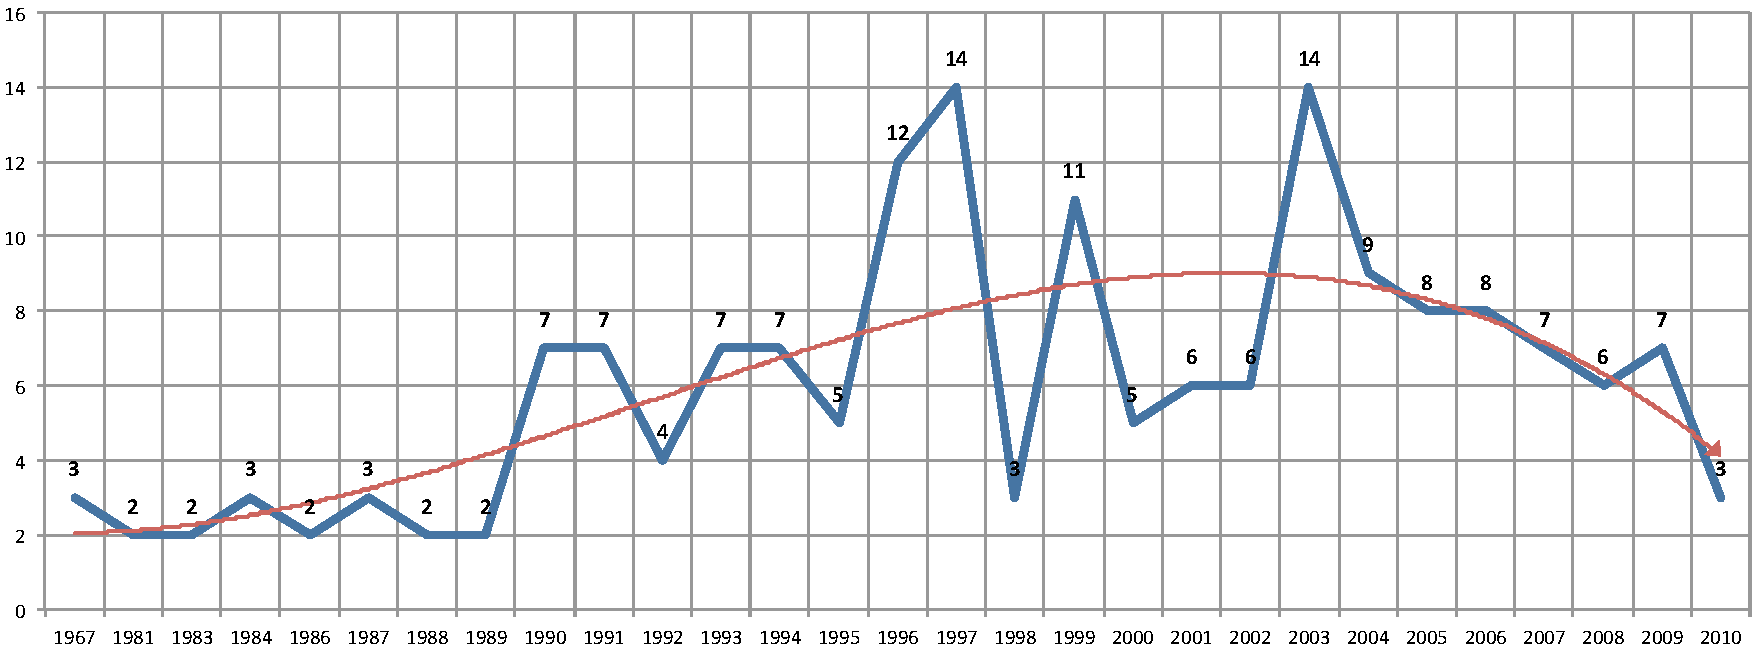
\includegraphics[scale=0.2]{/home/pfessel/abntex2/doc/latex/abntex2/abntex2-modelo-img-grafico}%
\end{minipage}\hfill{}%
\begin{minipage}[t]{0.4\textwidth}%
\caption{Gráfico 2 da minipage}
\label{fig-minipage-grafico2}

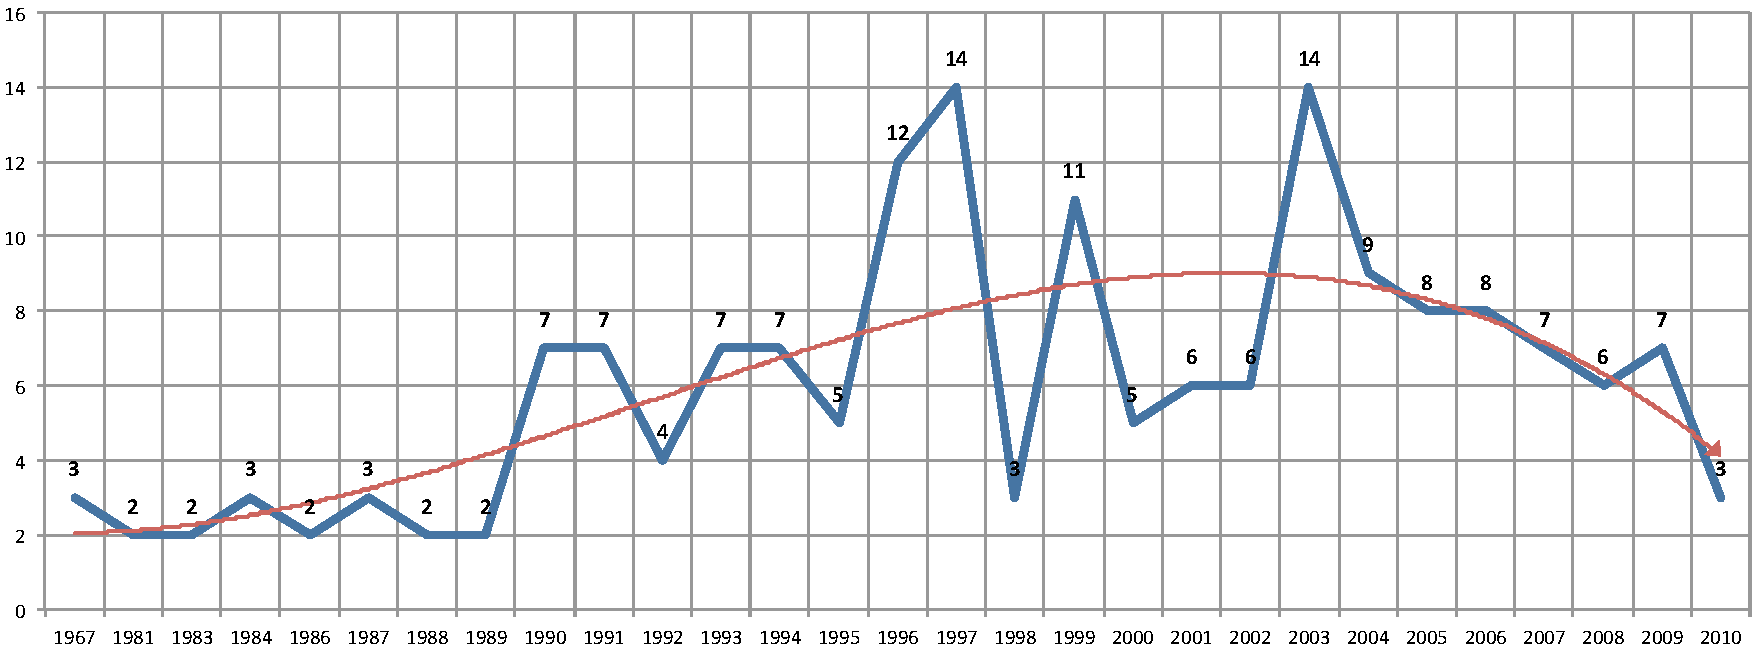
\includegraphics[scale=0.2]{/home/pfessel/abntex2/doc/latex/abntex2/abntex2-modelo-img-grafico}%
\end{minipage}
\end{figure}

\begin{citacao}
Qualquer que seja o tipo de ilustração, sua identificação aparece
na parte superior, precedida da palavra designativa (desenho, esquema,
fluxograma, fotografia, gráfico, mapa, organograma, planta, quadro,
retrato, figura, imagem, entre outros), seguida de seu número de ordem
de ocorrência no texto, em algarismos arábicos, travessão e do respectivo
título. Após a ilustração, na parte inferior, indicar a fonte consultada
(elemento obrigatório, mesmo que seja produção do próprio autor),
legenda, notas e outras informações necessárias à sua compreensão
(se houver). A ilustração deve ser citada no texto e inserida o mais
próximo possível do trecho a que se refere.\cite[seções 5.8]{NBR14724:2011}
\end{citacao}

\section{Equações matemáticas}

Um dos pontos muito fortes do \LyX{} é o seu editor de equações, que
é semalhante àqueles encontrados em programas de processamento de
texto como LibreOffice e Word. Ele pode ser acessado usando-se os
comandos ``Insert→Math''.

Equações numeradas são inseridas com ``Insert→Math→Numbered~Formula'':

\begin{equation}
\forall x\in X,\;\exists y\leq\epsilon
\end{equation}


Equações matemáticas também podem ser inseridas em linha com o comando
``Insert→Math→Inline\ Formula'', como por exemplo $\lim_{x\rightarrow\infty}\exp(-x)=0$.

Para inserir expressões matemáticas sem numeração, use o comando ``Insert→Math→Display\ Formula'':

\[
\left|\sum_{i=1}^{n}a_{i}b_{i}\right|\leq\left(\sum_{i=1}^{n}a_{i}^{2}\right)\left(\sum_{i=1}^{n}b_{i}^{2}\right)
\]


Consulte mais informações sobre expressões matemáticas em \url{http://code.google.com/p/abntex2/w/edit/Referencias}.


\section{Enumerações: alíneas e subalíneas}

\index{alíneas}\index{subalíneas}\index{incisos}Quando for necessário
enumerar os diversos assuntos de uma seção que não possua título,
esta deve ser subdividida em alíneas\cite[4.3]{NBR6024:2012}:
\begin{alineas}
\item os diversos assuntos que não possuam título próprio, dentro de uma
mesma seção, devem ser subdivididos em alíneas; 
\item o texto que antecede as alíneas termina em dois pontos;
\item as alíneas devem ser indicadas alfabeticamente, em letra minúscula,
seguida de parêntese. Utilizam-se letras dobradas, quando esgotadas
as letras do alfabeto;
\item as letras indicativas das alíneas devem apresentar recuo em relação
à margem esquerda;
\item o texto da alínea deve começar por letra minúscula e terminar em ponto-e-vírgula,
exceto a última alínea que termina em ponto final;
\item o texto da alínea deve terminar em dois pontos, se houver subalínea;
\item a segunda e as seguintes linhas do texto da alínea começa sob a primeira
letra do texto da própria alínea;
\item subalíneas \cite[4.3]{NBR6024:2012} devem ser conforme as alíneas
a seguir:

\begin{alineas}
\item as subalíneas devem começar por travessão seguido de espaço;
\item as subalíneas devem apresentar recuo em relação à alínea;
\item o texto da subalínea deve começar por letra minúscula e terminar em
ponto-e-vírgula. A última subalínea deve terminar em ponto final,
se não houver alínea subsequente;
\item a segunda e as seguintes linhas do texto da subalínea começam sob
a primeira letra do texto da própria subalínea.
\end{alineas}
\item no abn\TeX{} estão disponíveis os ambientes \texttt{incisos} e \texttt{subalineas},
que em suma são o mesmo que se criar outro nível de \texttt{alineas},
como nos exemplos à seguir:

\begin{incisos}
\item \textit{Um novo inciso em itálico;}
\end{incisos}
\item Alínea em \textbf{negrito}:

\begin{subalineas}
\item \textit{Uma subalínea em itálico;}
\item \textit{\uline{Uma subalínea em itálico e sublinhado;}}
\end{subalineas}
\item Última alínea com \emph{ênfase.}
\end{alineas}

\section{Espaçamento entre parágrafos e linhas}

\index{espaçamento!entre os parágrafos}O espaçamento entre um parágrafo
e outro pode ser controlado por meio do comando abaixo, inserido no
preâmbulo do documento (Document→Settings→Document\ Preamble):
\begin{lyxcode}
~\textbackslash{}setlength\{\textbackslash{}parskip\}\{0.2cm\}~~\%~tente~também~\textbackslash{}onelineskip
\end{lyxcode}
\index{espaçamento!entre as linhas}O controle do espaçamento entre
as linhas está disponível diretamente no menu de estilos, no grupo
``ABNTEXEspaços''. As opções são ``Simples'', ``1 e 1/2'' e
``Duplo''.


\section{Inclusão de outros arquivos\label{sec-include}}

É uma boa prática dividir o seu documento em diversos arquivos, e
não apenas escrever tudo em um único. Esse recurso foi utilizado neste
documento. Para incluir diferentes arquivos em um arquivo principal,
utilize o comando ``Insert→File→Child Document...''; para cada documento
filho, defina o documento mestre: isso é feito em ``Document→Settings→Document\ class''
selecionando-se a checkbox ``Select default master document''. Esse
comando funciona tanto com arquivos \LyX{}, \TeX{} ou \LaTeX{} (e
mesmo alguns outros), sempre lembrando que no caso dos documentos
\TeX{}/\LaTeX{} nenhuma verificação de sintaxe é feita; portanto,
você estará por sua própria conta e risco. Já arquivos \LyX{} podem
ser incluídos sem preocupações em relação à compatibilidade.


\section{Compilar o documento \protect\LaTeX{}}

No \LyX{}, os documentos são compilados com os comandos do menu ``View''.
Há atalhos de teclas para os formatos PDF (Ctrl-R) e DVI (Ctrl-D),
sendo que esses dois comandos compilam e exibem o resultado final
da compilação. Ctrl-Alt-R e Ctrl-Alt-D recompilam o documento, sem
no entanto solicitar uma nova janela para ele.

Caso seja necessário compilar os documentos do \LyX{} num \LaTeX{}
de linha de comando, deve-se usar o comando ``File→Export→\LaTeX{}
(pdflatex)'' e copiar todos os arquivos usados pelo documento mestre
num ú\pageref{chap:Resultados-de-comandos}nico diretório. Aí, para
compilar o documento, use os seguintes comandos:
\begin{lyxcode}
pdflatex~ARQUIVO\_PRINCIPAL~~~~

bibtex~ARQUIVO\_PRINCIPAL

makeindex~ARQUIVO\_PRINCIPAL.idx

makeindex~ARQUIVO\_PRINCIPAL.nlo~-s~nomencl.ist~-o~ARQUIVO\_PRINCIPAL.nls

pdflatex~ARQUIVO\_PRINCIPAL~~~~

pdflatex~ARQUIVO\_PRINCIPAL
\end{lyxcode}

\section{Remissões internas}

Ao nomear a \ref{tab-nvinv} e a \ref{fig-circulo}, apresentamos
um exemplo de remissão interna, que também pode ser feita quando indicamos
o \ref{chap:Resultados-de-comandos}, que tem o nome \emph{\nameref{chap:Resultados-de-comandos}}.
O número do capítulo indicado é \prettyref{chap:Resultados-de-comandos},
que se inicia à \pageref{chap:Resultados-de-comandos}%
\footnote{O número da página de uma remissão pode ser obtida também assim: \textbackslash{}pageref\{cap\_exemplos\}.%
}. Veja a \ref{sec-divisoes} para outros exemplos de remissões internas
entre seções, subseções e subsubseções.


\section{Divisões do documento: seção\label{sec-divisoes}}

Esta seção testa o uso de divisões de documentos. Esta é a \ref{sec-divisoes}.
Veja a \ref{sec-divisoes-subsection}.


\subsection{Divisões do documento: subseção\label{sec-divisoes-subsection}}

Isto é uma subseção. Veja a \ref{sec-divisoes-subsubsection}, que
é uma \texttt{subsubsection} do \LaTeX{}, mas é impressa chamada de
``subseção'' porque no Português não temos a palavra ``subsubseção''.


\subsubsection{Divisões do documento: subsubseção\label{sec-divisoes-subsubsection}}

Isto é uma subsubseção.


\subsubsection{Divisões do documento: subsubseção}

Isto é outra subsubseção.


\subsection{Divisões do documento: subseção\label{sec-exemplo-subsec}}

Isto é uma subseção.


\subsubsection{Divisões do documento: subsubseção}

Isto é mais uma subsubseção da \ref{sec-exemplo-subsec}.


\paragraph{Isto é um parágrafo rotulado\label{sec-exemplo-paragrafo}}


\paragraph{Este é um parágrafo na \ref{sec-exemplo-paragrafo}. }


\paragraph{Isto é outro parágrafo rotulado\label{sec-exemplo-paragrafo-outro}}


\paragraph{Este é outro parágrafo na \ref{sec-exemplo-paragrafo-outro}. }


\section{Este é um exemplo de nome de seção longo. Ele deve estar alinhado
à esquerda e a segunda e demais linhas devem iniciar logo abaixo da
primeira palavra da primeira linha}

Isso atende à norma \textbackslash{}citeonline{[}seções de 5.2.2 a
5.2.4{]}\{NBR14724:2011\} e \textbackslash{}citeonline{[}seções de
3.1 a 3.8{]}\{NBR6024:2012\}.


\section{Diferentes idiomas e hifenizações\label{sec-hifenizacao}}

Para usar hifenizações de diferentes idiomas, inclua nas opções do
documento o nome dos idiomas que o seu texto contém. Por exemplo:
\begin{lyxcode}
\textbackslash{}documentclass{[}12pt,openright,twoside,a4paper,english,french,spanish,brazil{]}\{abntex2\}
\end{lyxcode}
A lista completa de idiomas suportados, bem como outras opções de
hifenização, estão disponíveis em \textbackslash{}citeonline{[}p.\textasciitilde{}5-6{]}\{babel\}.

Exemplo de hifenização em inglês%
\footnote{Extraído de: \url{http://en.wikibooks.org/wiki/LaTeX/Internationalization}%
}:

\selectlanguage{english}%
\textit{Text in English language. This environment switches all language-related
definitions, like the language specific names for figures, tables
etc. to the other language. The starred version of this environment
typesets the main text according to the rules of the other language,
but keeps the language specific string for ancillary things like figures,
in the main language of the document. The environment hyphenrules
switches only the hyphenation patterns used; it can also be used to
disallow hyphenation by using the language name `nohyphenation'.}

\selectlanguage{brazil}%
Exemplo de hifenização em francês%
\footnote{Extraído de: \url{http://bigbrowser.blog.lemonde.fr/2013/02/17/tu-ne-tweeteras-point-le-vatican-interdit-aux-cardinaux-de-tweeter-pendant-le-conclave/}%
}:

\selectlanguage{french}%
\textit{Texte en français. Pas question que Twitter ne vienne faire
une concurrence déloyale à la traditionnelle fumée blanche qui marque
l'élection d'un nouveau pape. Pour éviter toute fuite précoce, le
Vatican a donc pris un peu d'avance, et a déjà interdit aux cardinaux
qui prendront part au vote d'utiliser le réseau social, selon Catholic
News Service. Une mesure valable surtout pour les neuf cardinaux –
sur les 117 du conclave – pratiquants très actifs de Twitter, qui
auront interdiction pendant toute la période de se connecter à leur
compte.}

\selectlanguage{brazil}%
Pequeno texto em espanhol%
\footnote{Extraído de: \url{http://internacional.elpais.com/internacional/2013/02/17/actualidad/1361102009_913423.html}%
}:

\selectlanguage{spanish}%
\textit{Decenas de miles de personas ovacionan al pontífice en su
penúltimo ángelus dominical, el primero desde que anunciase su renuncia.
El Papa se centra en la crítica al materialismo.}\selectlanguage{brazil}%

\end{document}


\bibliographystyle{abntex2-alf}
\bibliography{/home/pfessel/abntex2/doc/latex/abntex2/abntex2-doc,/home/pfessel/abntex2/doc/latex/abntex2/abntex2-modelo-references}

\end{document}
